\documentclass[11pt, a4paper, twoside, openright]{book} %draft

\usepackage{graphicx,color}
\usepackage{amssymb, amsmath, array}
\usepackage{epigraph}
\usepackage[font=small,labelfont=bf]{caption}

% \epigraphsize{\small}% Default
\setlength\epigraphwidth{8cm}
\setlength\epigraphrule{0pt}



\begin{document}

% Example of title page for the projects carried out within DEDIS
% Copied from lasec 

% Simply include it in your mastex tex file: 
%        % Example of title page for the projects carried out within DEDIS
% Copied from lasec 

% Simply include it in your mastex tex file: 
%        % Example of title page for the projects carried out within DEDIS
% Copied from lasec 

% Simply include it in your mastex tex file: 
%        \input{cover}


% Updated October 2016


\newcommand{\logoepfl}[0]{
  \begin{center}
    
\includegraphics[width=4cm]{logo_epfl_coul.eps}
  \end{center}
  \vspace{0.3cm}
  \hrule
}
\newcommand{\project}[1]{
  \begin{center}
    \large{#1}
  \end{center}
  \vspace{1cm}
}
\newcommand{\department}[1]{
  \begin{center}
    \large{#1}
  \end{center}
}
\newcommand{\lab}[1]{
  \begin{center}
    \large{#1}
  \end{center}
}
\newcommand{\supervisor}[3]{
  \begin{center}
    \begin{normalsize}{
        \bf #1}\\#2\\#3
    \end{normalsize}
  \end{center}
}
\renewcommand{\author}[1]{
  \begin{center}
    \Large{#1}
  \end{center}
  \vspace{0.5cm}
}
\renewcommand{\title}[1]{
  \vspace{3cm}
  \begin{center}
    \huge{#1}
  \end{center}
  \vspace{1.7cm}
}
\renewcommand{\date}[2]{
  \begin{center}
    \normalsize{#1 #2}
  \end{center}
  \vspace{0.5cm}
}


\thispagestyle{empty}




% begin title page
  \logoepfl
  
  \title{Proof of Personhood tokens on the ethereum blockchain}
  
  \author{Hugo Roussel}
  \department{School of Computer and Communication Sciences}
  \lab{Decentralized and Distributed Systems lab}
  \project{Bachelor Project}
  
  \date{December}{2017}

  \begin{center}
    \begin{tabular}{cc}
      \begin{tabular}{p{4.0cm}}
        \supervisor{Responsible}{Prof. Bryan Ford}{EPFL / DEDIS}
      \end{tabular}&
      \begin{tabular}{p{4.0cm}}
        \supervisor{Supervisor}{Linus Gasser}{EPFL / DEDIS}
      \end{tabular}
    \end{tabular}
  \end{center}
  

  

% end title page




% Updated October 2016


\newcommand{\logoepfl}[0]{
  \begin{center}
    
\includegraphics[width=4cm]{logo_epfl_coul.eps}
  \end{center}
  \vspace{0.3cm}
  \hrule
}
\newcommand{\project}[1]{
  \begin{center}
    \large{#1}
  \end{center}
  \vspace{1cm}
}
\newcommand{\department}[1]{
  \begin{center}
    \large{#1}
  \end{center}
}
\newcommand{\lab}[1]{
  \begin{center}
    \large{#1}
  \end{center}
}
\newcommand{\supervisor}[3]{
  \begin{center}
    \begin{normalsize}{
        \bf #1}\\#2\\#3
    \end{normalsize}
  \end{center}
}
\renewcommand{\author}[1]{
  \begin{center}
    \Large{#1}
  \end{center}
  \vspace{0.5cm}
}
\renewcommand{\title}[1]{
  \vspace{3cm}
  \begin{center}
    \huge{#1}
  \end{center}
  \vspace{1.7cm}
}
\renewcommand{\date}[2]{
  \begin{center}
    \normalsize{#1 #2}
  \end{center}
  \vspace{0.5cm}
}


\thispagestyle{empty}




% begin title page
  \logoepfl
  
  \title{Proof of Personhood tokens on the ethereum blockchain}
  
  \author{Hugo Roussel}
  \department{School of Computer and Communication Sciences}
  \lab{Decentralized and Distributed Systems lab}
  \project{Bachelor Project}
  
  \date{December}{2017}

  \begin{center}
    \begin{tabular}{cc}
      \begin{tabular}{p{4.0cm}}
        \supervisor{Responsible}{Prof. Bryan Ford}{EPFL / DEDIS}
      \end{tabular}&
      \begin{tabular}{p{4.0cm}}
        \supervisor{Supervisor}{Linus Gasser}{EPFL / DEDIS}
      \end{tabular}
    \end{tabular}
  \end{center}
  

  

% end title page




% Updated October 2016


\newcommand{\logoepfl}[0]{
  \begin{center}
    
\includegraphics[width=4cm]{logo_epfl_coul.eps}
  \end{center}
  \vspace{0.3cm}
  \hrule
}
\newcommand{\project}[1]{
  \begin{center}
    \large{#1}
  \end{center}
  \vspace{1cm}
}
\newcommand{\department}[1]{
  \begin{center}
    \large{#1}
  \end{center}
}
\newcommand{\lab}[1]{
  \begin{center}
    \large{#1}
  \end{center}
}
\newcommand{\supervisor}[3]{
  \begin{center}
    \begin{normalsize}{
        \bf #1}\\#2\\#3
    \end{normalsize}
  \end{center}
}
\renewcommand{\author}[1]{
  \begin{center}
    \Large{#1}
  \end{center}
  \vspace{0.5cm}
}
\renewcommand{\title}[1]{
  \vspace{3cm}
  \begin{center}
    \huge{#1}
  \end{center}
  \vspace{1.7cm}
}
\renewcommand{\date}[2]{
  \begin{center}
    \normalsize{#1 #2}
  \end{center}
  \vspace{0.5cm}
}


\thispagestyle{empty}




% begin title page
  \logoepfl
  
  \title{Proof of Personhood tokens on the ethereum blockchain}
  
  \author{Hugo Roussel}
  \department{School of Computer and Communication Sciences}
  \lab{Decentralized and Distributed Systems lab}
  \project{Bachelor Project}
  
  \date{December}{2017}

  \begin{center}
    \begin{tabular}{cc}
      \begin{tabular}{p{4.0cm}}
        \supervisor{Responsible}{Prof. Bryan Ford}{EPFL / DEDIS}
      \end{tabular}&
      \begin{tabular}{p{4.0cm}}
        \supervisor{Supervisor}{Linus Gasser}{EPFL / DEDIS}
      \end{tabular}
    \end{tabular}
  \end{center}
  

  

% end title page




\newpage

\section{Introduction}
A current problem on internet is that it's impossible to concile anonymity and accountability. Imagine an internet forum where users wish to share their political views anonymously but still wish to avoid "trolls", members that don't add value to the discussion. It's always possible to block an anonymous account but the "troll" can create a new one easily. This is not a viable solution. The forum could block certain IP addresses but once again it suffices for the troll to use a VPN or another connection. Another solution would be to ask each new member to provide an ID and verify their identity, however the discussion isn't anonymous anymore. \\
We will explain in the following paper a way to reconcile free speech and responsability and one implementation of it : Proof of Persoonhood tokens.



\section{Proof of Personhood tokens}
\subsection{What are Proof of Personhood tokens?}

\epigraph{``Accountable anonymous credentials``}
{--- \textup{Proof-of-Personhood: Redemocratizing Permissionless Cryptocurrencies}}

Proof of personhood tokens associate one person with one token. Binding a physical identity with a digital identity. The results can be achievied by combining pseudonym parties and cryptographic tools.

\subsection{Pseudonym parties}

The idea behind a pseudonym party is to verify persons and not identities. A party goes as follows :  attendees met at designed location. Each attendees deposits a public key and once done, the key is added to the set of key of other participants. The person then is marked using permanent marker to insure he doesn't deposit twice. Once each attendee had the chance to register, the party ends and the organizers release the final statement of the party : the keyset of all participants along with details of the party. For transparency purposes the party can be fimed, in that case the hash of the tape is added to the final statement. 
 
\subsection{Current implementation}
The current DEDIS implementation of PoP tokens is implemented using Golang on the Skipchain. The Skipchain is a blockchain created at EPFL by the DEDIS laboratory. The service provides commands for organizers and attendees to link to the skipchain for interacting with it 

\subsection{Limitations}
For the moment skipchain is a private blockchain, meaning that only certified nodes can be added to it. The motivation of the project was to port the service to a public blockchain where ultimately it could be useful to more users. 

\section{Ethereum}

\subsection{Ethereum, Solidity and smart contracts}
 Ethereum is an open-source public blockchain which can perform decentralized computations on the ethereum virtual machine. The EVM is a worldwide computer than anyone can use is exchange for a small fee payed in the crypto-currency of the platform, ether. Scripts running on the EVM are called "smartcontracts". They must be written in Solidity a statically-typed programming language inspired in its syntax of Javascript. Solidity is compiled to bytecode that is then pushed to the EVM. 


\subsection{Why use Ethereum?}

\epigraph{The value of a network is proportional to the square of the number of connected users of the system}
{--- \textup{Metacalfe's law}}

The ethereum platform quickly gained in popularity after its launch. The ecosystem has many tools to intereact with the blockchain and to create decentralized applications. It is currently the network with the most nodes making it more secure and less centralized. A public blockchain also provides a greater transparency as every actor can verify who intereact and how with the contract. This can be done easily using a block explorer. 
\newpage



\section{Implementation of Popcontract}
The popcontract is a smart-contract used to organize and store the informations of pseudonym party. It is modeled by a finite state machine to improve security and reliability.
\subsection{Abstract}
Create a smart-contract that will store the information of the pseudonym party. At the end of the party, the contract is then locked, rendering it immuable. Each user can then refer to it knowing its genuinity.
Then make the system interoperable with the current DEDIS implementation to have a clear and easy to use interface.   


  
  \begin{minipage}{1\linewidth}
    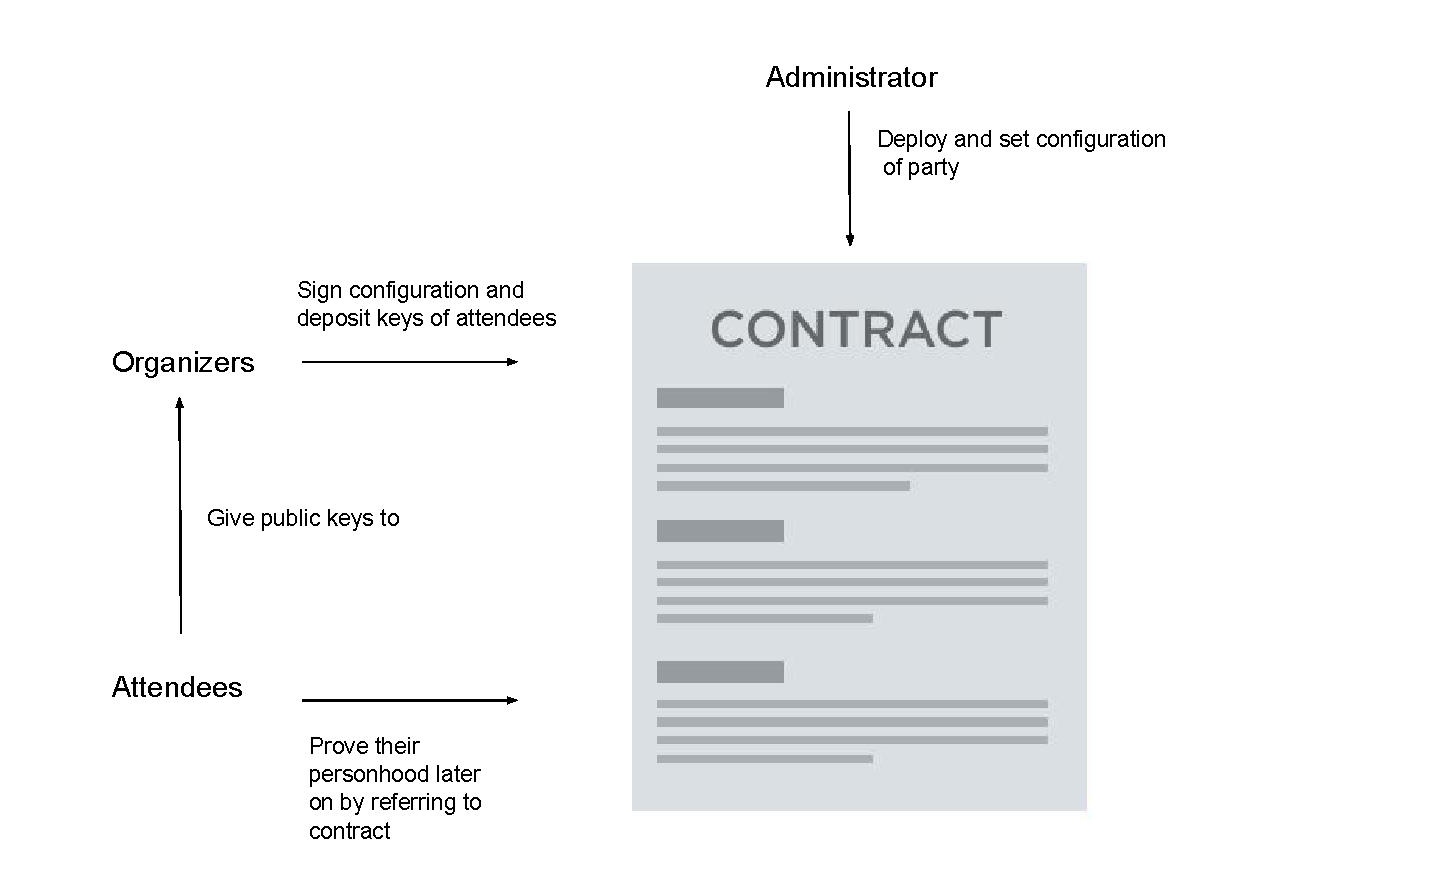
\includegraphics[scale = 0.67]{popcontract.pdf}
\captionof{figure}{How actors intereact with contract}
\end{minipage}%
  
\subsection{Popcontract finite state machine}
An easy way to improve security of a smart contract is to transform it into a finite state machine (FSM). Thus at each state only certain functions can be called. This reduce the risk that some functions will be called maliciously.\\ The contract is modeled by a FSM with only five state : \\- initial state (contract was succefully deployed)\\ - configurationSet state (administrator provided the details of the party) \\ - configurationSigned state (organizers agree with the configuration) \\ - key-deposited state (at least one keyset was sent to contract)\\ - locked (party ended and final keyset was choosed)

\begin{minipage}{1\linewidth}
    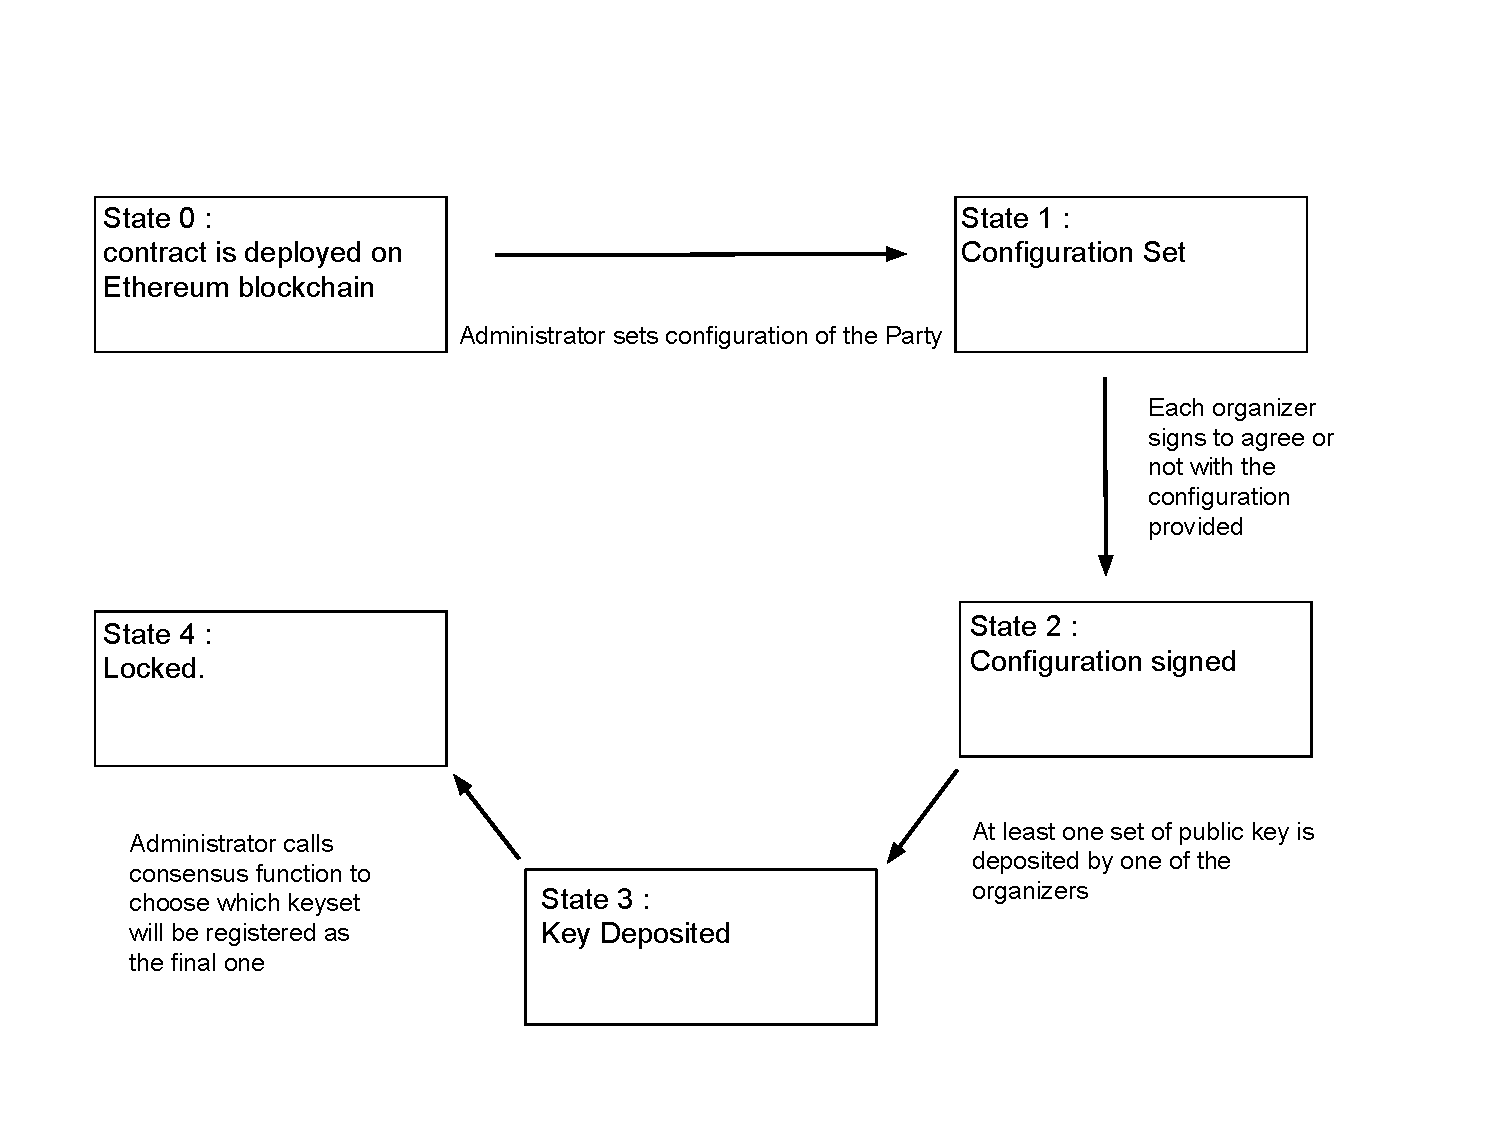
\includegraphics[scale = 0.67]{fsm.pdf}
\captionof{figure}{Popcontract FSM}
\end{minipage}%

\subsection{Technical implementation}
\subsubsection{Configuration of party}
The configuration of the party is defined as follows : a name, a location, an array of public keys of organizers (in ethereum format) as well as a deadline. Passed the deadline, no function of the contract is callable, renforcing security. The administrator sends a transaction signed with its private key with all the information above. The administrator is defined as the person holding the private key used to deploy the contract initially. Of course the administrator must have enough ether/test-ether to pay the fee. 
\subsubsection{Signing of configuration}
 To prevent a single entity (the administrator) controlling the contract, all the organizers have to sign the configuration by sending a transaction signed with their private key to the contract. While the configuration is not fully signed by all organizers, no keys can be deposited.
\subsubsection{Deposit of public keys of attendees}  
 The organizers then send a set of public key to the contract using a transaction signed with their private key including the data they wish to push. The current key format supported for attendees is ed25519 to permit interoperability with the first implementation.
\subsubsection{Consensus and lock}
Once at least one keyset is added, the administrator can call a consensus function that will lock the contract and will choose which keyset will be considered as the "official" keyset.


\subsection{How to interact with an Ethereum smartcontract}
A deployed smart contract is defined by it's address and it's ABI (Application Binary Interface). You can get the ABI of a contract using the Solidity compiler.
\subsubsection{Creating and sending transactions}
A transaction is a call to the EVM to intereact with a contract or an account. Technically a transaction should be from human to human and a message is human to contract or contract to contract. For clarity purposes we will not do the distinction and only use the term transaction. A transaction is constitued of the following fields : \\
- recipient address (contract or human) \\
- signature identifying the sender \\
- value field for transfer of ether. Here this field will always be ignored.\\
- gas limit, the maximum fee the sender is ready to pay \\
- gas price, decided by miners \\
- nonce, the number of transactions made by the account to avoid replay attacks\\
- data field \\

It's possible to create raw transactions through a node.js console attached to the network.


\subsubsection{Other ways}
Many tools exist to intereact with the ethereum blockchain, we will cite the most popular : \\
- Mist browser, official application that serves both as a wallet and a way to deploy smart-contract and intereact with them. You will need to run a full node (download the whole blockchain) to use it or connect to another node.\\
- Myetherwallet.com website that serves as a wallet and way to intereact with smart contract. The website is connected to a node and send transactions created on the website to the network.



\subsection{Interoperability with current system}


\section{Theoretical and practical limitations of the implementation.}
\section{Results}
\section{Possible improvements}
\section{How to create PoP tokens using the contract}

 


\section{What to do}


Introduction of the subject and the problem.
Goals of the project and motivation.
Corresponding background.
Step-by-step description of your design/implementation/evaluation/analysis.
Theoretical and practical limitations of the project and its implementation.
Results.
Evaluation of the results and comparison with other approaches if applicable.
Future work.
Step-by-step guide for installation, including dependecies, and running of the final product.








\end{document}
